\newcommand\SCALE{0.47}

% \section{Introduction}

Peer-sampling
protocols~\cite{jelasity2007gossip,tolgyeski2009adaptive,voulgaris2005cyclon}
constitute a fundamental mechanism for a number of large-scale distributed
applications both on the Cloud~\cite{decandia2007dynamo} and in a peer-to-peer
setting~\cite{Frey09Middleware,voulgaris2005sub,wuhib2009robust}. By providing
each node with a continuously changing partial view of the network, they make
applications resilient to churn~\cite{bertier-d2ht} and inherently load
balancing~\cite{Frey09DSN}. In the context of video streaming, for example, a
peer-sampling protocol makes it possible to distribute the streaming load over
all peers without requiring the creation and the maintenance of rigid structures
like multiple trees~\cite{Frey09DSN,monod:THESIS}.

The recent introduction of WebRTC~\cite{webrtc} has renewed the
research interest in a variety of applications that require
peer-sampling protocols such as video streaming~\cite{hivejs,smoothcache2},
content-delivery networks~\cite{Zhang:2013:MBC:2465351.2465379}, or
real-time collaborative editors~\cite{nedelec2016crate}. However,
deploying existing peer-sampling protocols on top of WebRTC raises
important technical challenges.
\begin{inparaenum}[(1)]
\item WebRTC does not manage addressing nor routing; this makes
  connection establishment much more costly than on IP networks and
  more likely to fail. 
\item Browsers run on desktops, laptops and mobile phones. This
  requires protocols that reduce resource consumption as much as
  possible.
\item The ability to launch WebRTC sessions through simple HTTP links
  exposes applications to sudden bursts of popularity.
\end{inparaenum}
Consider the example of a user who is streaming a video directly from
his mobile phone to some of his friends. The user suddenly witnesses
some dramatic event, and his friends spread the news by twitting the
stream's address. Instantly a huge number of users connect and start
watching the stream on their laptops and phones. The streaming
mechanisms and the protocols it relies on must be able to adapt to
this sudden burst of popularity, maintaining their quality of service,
while being able to return to their initial configuration when the
popularity burst subsides. 

Unfortunately, existing peer-sampling protocols lack adaptiveness or
reliability in the context of WebRTC. On the one hand,
\SCAMP~\cite{ganesh2001scamp,ganesh2003peer} provides adaptiveness by
maintaining partial views of size $\ln(n)+k$, $n$ being the number of
nodes and $k$ being a constant. However, \SCAMP is not reliable in the
context of WebRTC, for its connection establishment process is based
on random walks and cannot handle the connection failures that often
occur in WebRTC. On the other hand, the most popular approaches like
\CYCLON~\cite{voulgaris2005cyclon} and the whole RPS protocol
family~\cite{jelasity2007gossip} are reliable in the context of WebRTC
but are not adaptive: developers have to configure fixed-size views at
deployment time. This forces developers to oversize partial views to
handle potential bursts, either wasting resources or not provisioning
for large-enough settings. A simple solution to address this problem
estimates the actual number of network nodes by periodically running
an aggregation protocol~\cite{montresor2004robust}, then resizes the
partial views. However, this aggregation protocol would have to run
quite frequently, resulting in significant network overhead to
anticipate a popularity burst that may never happen. Our approach
provides adaptiveness and reliability by locally self-adjusting the
size of partial views at join, leave, and shuffle times. At a marginal
cost, partial view size converges towards $\ln(n)$. This not only
makes our approach adaptive but also outputs the size of the network
to the application level allowing applications to adapt to sudden
burst in popularity at no additional cost. We demonstrate the impact
of our approach on two use cases that use RPS to broadcast
messages. The first one implements a live video streaming based on
three-phase gossip~\cite{Frey09DSN,FlightPath,monod:THESIS}. In this
case, adaptiveness allows message delivery to remain stable even in
presence of burst in popularity. The second one implements a real-time
collaborative editor. In this case, adaptiveness allows the editors to
adjust the traffic to the size of the network. Some distributed hash
table protocols such as D2HT~\cite{bertier-d2ht} require both the
knowledge of the size of the network to compute the view of each node,
and a random peer-sampling protocol to provide connectivity in the
presence of high churn. Our approach provides both at the same cost.

% The scientific challenge consists in finding a way to adapt to the
% network size without actually measuring its number of members as
% proposed by Scamp, but running on top of WebRTC.

%% In this paper, 
We address the challenge of a dynamically adaptive peer-sampling,
by introducing \SPRAY, a novel random peer-sampling protocol inspired by both
\SCAMP~\cite{ganesh2001scamp,ganesh2003peer} and
\CYCLON~\cite{voulgaris2005cyclon}. \SPRAY improves the state-of-the-art in
several ways.

\begin{figure}
  \begin{center}
    \subfloat[Figure A] [add $1+\ln(n)$ links]
    {
\scalebox{1.3}{
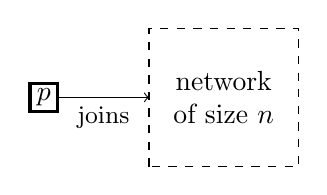
\begin{tikzpicture}

  \newcommand\X{65pt};
  \newcommand\Y{15pt};


  \draw[->] (5+0*\X, 0*\Y) -- node[anchor=north]{\small{joins}} (-27+1*\X, 0*\Y);

  \draw[fill=white, very thick]
  (0*\X, 0*\Y) node{$p$} +(-5pt,-5pt) rectangle +(5pt,5pt);
  

  \draw[fill=white, dashed]
  (1*\X, 0*\Y) node[align=center]{network\\of size $n$} +(-27pt,-25pt) rectangle +(27pt,25pt);

 
\end{tikzpicture}
}}
    \hspace{20pt}
    \subfloat[Figure B] [constant number of links]
    {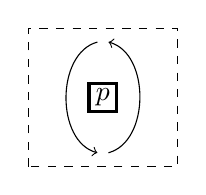
\begin{tikzpicture}{scale=1.5}

  \newcommand\X{65pt};
  \newcommand\Y{15pt};


%  \draw[->] (0*\X, 0*\Y) -- node{rejoint} (-27+1*\X, 0*\Y);


  \draw[fill=white, dashed]
  (0*\X, 0*\Y) +(-27pt,-25pt) rectangle +(27pt,25pt);

  \draw[fill=white, very thick]
  (0*\X, 0*\Y) node{$p$} +(-5pt,-5pt) rectangle +(5pt,5pt);
  
  \draw[->] (  2+0*\X, -20+0*\Y ) to[out=15,in=-15] (2+0*\X, 20+0*\Y);
  \draw[<-] ( -2+0*\X, -20+0*\Y ) to[out=165,in=-165] (-2+0*\X, 20+0*\Y);

 
\end{tikzpicture}}
    \hspace{20pt}
    \subfloat[Figure C] [remove $1+\ln(n)$ links]
    {
\scalebox{1.3}{
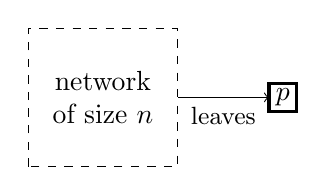
\begin{tikzpicture}

  \newcommand\X{65pt};
  \newcommand\Y{15pt};


  \draw[->] (27+0*\X, 0*\Y) -- node[anchor=north]{\small{leaves}} (-5+1*\X, 0*\Y);

  \draw[fill=white, very thick]
  (1*\X, 0*\Y) node{$p$} +(-5pt,-5pt) rectangle +(5pt,5pt);
  

  \draw[fill=white, dashed]
  (0*\X, 0*\Y) node[align=center]{network\\of size $n$}
  +(-27pt,-25pt) rectangle +(27pt,25pt);

 
\end{tikzpicture}
}}
    \caption{\label{fig:cycle} Life cycle of a peer.}
  \end{center}
\end{figure}

\paragraph{Adaptive.}
Peers using \SPRAY see their neighborhood size growing and shrinking
automatically regarding the global network size using local knowledge only. In
addition, the neighborhood size scales logarithmically compared to the network
size. Figure~\ref{fig:cycle} shows that \SPRAY achieves this by dividing the
life cycle of a peer in 3 phases:
\begin{enumerate}[(i)]
\item When a peer \emph{joins}, we must add logarithmic number of links to the
  network. The peer joins using a contact peer already inside the network. This
  contact has a neighborhood the size of which is the logarithm of the network
  size. The contact simply asks to its neighbors to establish a link with the
  newcomer to get the proper global number of arcs.
\item When a peer stays in the network, it periodically \emph{shuffles} its
  neighborhood with one of its current neighbor. During shuffles, the global
  number of arcs must remain constant. Involved peers give a part of their
  neighborhood. They remove the link to given neighbors and the other involved
  peer must create a link to these. Shuffles may create duplicated links that
  must be temporarily kept.  Over shuffles, the number of duplicates remains
  small compared to the network size and becomes negligible as the network
  grows.
\item When a peer \emph{crashes} or \emph{leaves}, we must remove a logarithmic
  number of links. This number must match the number of links added during the
  joining phase of the newest peer. Unfortunately, these departures leads to an
  overzealous removal of links. To fix the number of arcs, all but one of the
  peers that have the departed peer in their neighborhood should create a
  duplicated link. Since they do not know each other, they cannot
  communicate. They use their neighborhood size to process the probability of
  duplicating.
\end{enumerate}

Figure~\ref{fig:extended} shows the results of an experiment where 4 distinct
networks of size have a membership continuously oscillating from 50k to 100k peers, 5k
to 10k peers, 500 to 1k peers, and 50 to 100 peers. We measure the average
partial view size of peers. We see that
\begin{inparaenum}[(i)]
\item the measures are not far from the theoretical values (dashed);
\item the partial view sizes vary reflecting the network size;
\item the values are more stable when the network is large.
\end{inparaenum}


%\TODO{formula harmonic number.}


\begin{figure}
  \begin{center}
    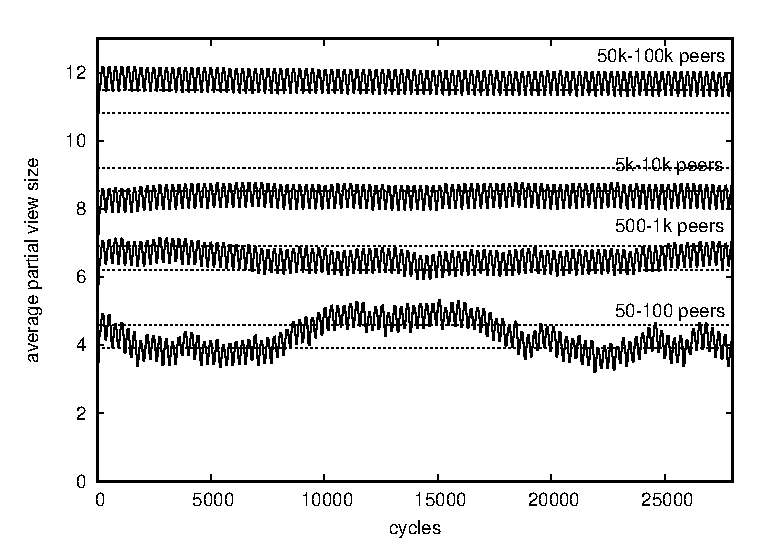
\includegraphics[width=\SCALE\textwidth]{./img/extended.eps}
    \caption{\label{fig:extended} Neighborhoods grow and shrink reflecting the
      changes of network size.}
  \end{center}
\end{figure}

%% It dynamically adapts the neighborhood of each peer. Thus, the number of
%% connections scales logarithmically with the network size.

\paragraph{Cautious.}
All along the life cycle of a peer, it uses simple neighbor-to-neighbor
interactions to create links.  Peers rely on a constant number of other nodes to
create links regardless of network size. The chances to execute backup
strategies due to network failures -- message losses or peer crashes -- are kept
minimal.

\paragraph{Fast.}
The network quickly converges to a topology with properties similar to those of
random graphs. The clustering coefficient is low. The incoming and outgoing arcs
numbers are balanced among peers. There exists no hubs nor weakly connected
peers. The network becomes robust to massive failures. The average shortest path
length grows logarithmically. It can quickly disseminate messages.


% \begin{figure}
%   \begin{center}
%     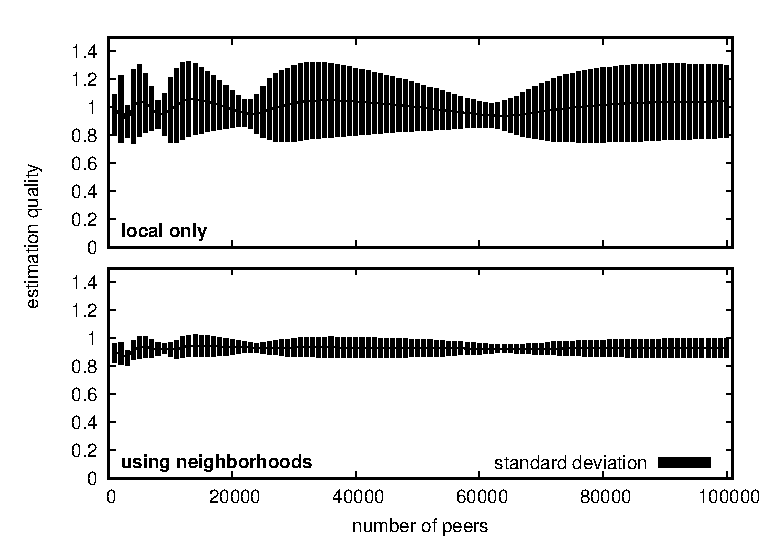
\includegraphics[width=\SCALE\textwidth]{./img/estimator.eps}
%     \caption{\label{fig:estimator} The quality of the network size estimator
%       based on neighborhood size.}
%   \end{center}
% \end{figure}



\ \\ \indent \SPRAY alone provides all desirable properties of random peer-sampling
protocols. It maintains a connected topology even in presence of massive network
failures. In addition, its neighborhood size provides an insight of the network
size. Protocols and applications can benefit of this feature. Firstly, we show
the accuracy of a network size estimator using partial view sizes. Secondly, we
provide 2 examples of broadcast protocols.


\begin{figure}
  \begin{center}
    \subfloat[Figure A] [\label{fig:estimator} The quality of the network 
    size estimator based on neighborhood size.]
    {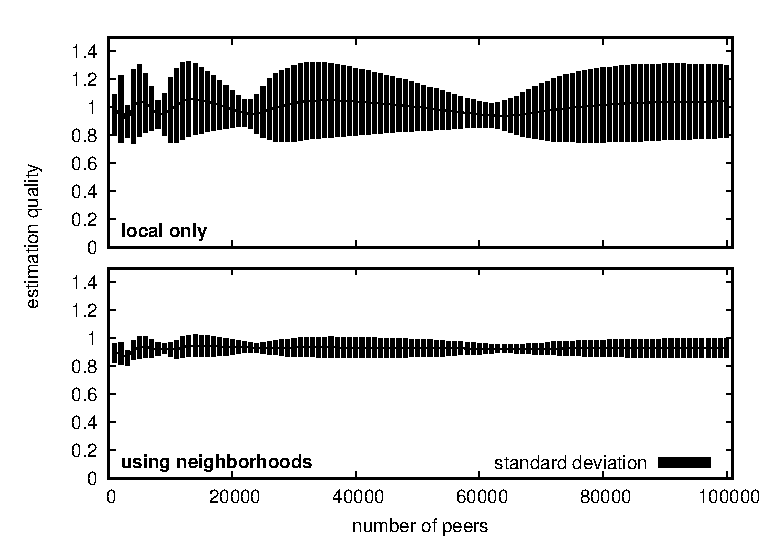
\includegraphics[width=\SCALE\textwidth]{img/estimator.eps}}\\
    \subfloat[Figure B] [\label{fig:hardrate} Full message delivery in
    three-phases broadcast.]
    {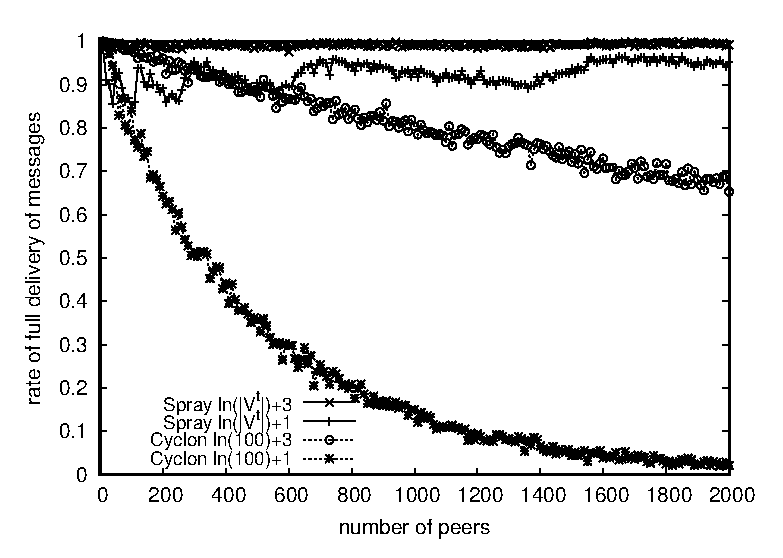
\includegraphics[width=\SCALE\textwidth]{img/hardrate.eps}}    
    \subfloat[Figure C] [\label{fig:traffic} Outgoing traffic generated by a
    real-time collaborative editing.]
    {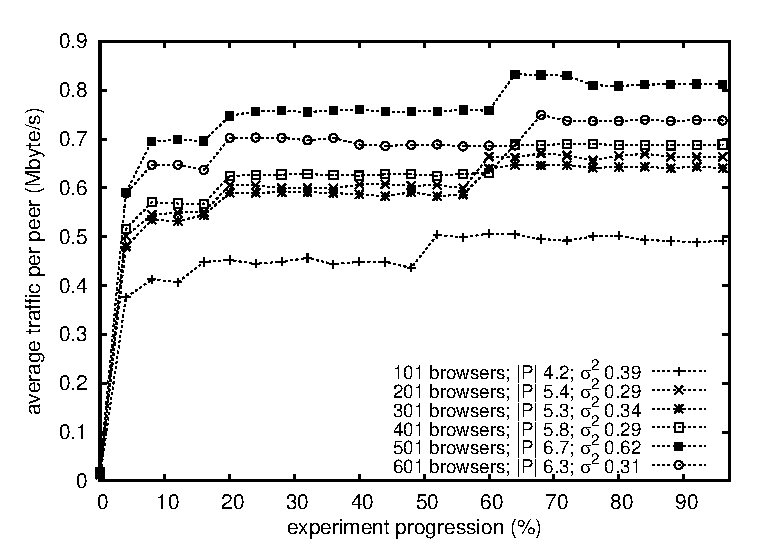
\includegraphics[width=\SCALE\textwidth]{img/traffic.eps}}
    \caption{Example of applications benefiting from \SPRAY.}
  \end{center}
\end{figure}

\paragraph{Estimator.} Figure~\ref{fig:estimator} shows the results of
measurements concerning the average estimation of network size over the actual
network size. The estimator either uses the local partial view size only or the
local view plus the view size of its neighbors. We see that
\begin{inparaenum}[(i)]
\item the estimation is close to the actual network size and
\item using neighborhood, the estimation can be improved.
\end{inparaenum}
This means that an application can improve its estimation on demand depending on
the available resources.

\paragraph{Three-phases broadcast.} Figure~\ref{fig:hardrate} shows the results
of measurements concerning the proportion of messages delivered to the whole
network over 1k messages. The network grows over time. We compare a broadcast
that adjusts its fanout (the number of neighbors it sends/forwards a message to)
using the partial view size (\SPRAY), and a fanout configured in advance
(\CYCLON). We see that
\begin{inparaenum}
\item when configured in advance, the full message delivery quickly drops as the
  network size increases; 
\item on the opposite, when the fanout adjusts to the adaptive partial view
  size, the full message delivery stays relatively stable.
\end{inparaenum}
This means that applications that requires full delivery can rely on
\SPRAY-based broadcast to bound the reliability of message delivery whatever the
network size.


\paragraph{Reliable broadcast.} Figure~\ref{fig:traffic} shows the results of
measurements concerning the traffic generated by decentralized collaborative
editing. \TODO{Not done here.}

\SPRAY makes building scalable decentralized applications in browsers easy and
accessible.  Developers do not require to foresee the network size targeted by
their applications. Just the same as for broadcast, many topology optimization
protocols (e.g. about geolocalization, latency, or preferences) rely on random
peer-sampling protocol such as the generic algorithms
T-Man~\cite{jelasity2009tman} and Vicinity~\cite{voulgaris2005epidemic}. \SPRAY
allows such protocols to benefit from its self-adjusting partial
views. Protocols such as D2HT~\cite{bertier-d2ht} require both an estimator of
the network size and a random peer-sampling protocol. Since \SPRAY provides both
at same cost, a \SPRAY-based D2HT would be an interesting perspective.

% \begin{inparaenum}[(i)]
% \item Experiments show that \SPRAY provides adaptiveness and reliability at a
%   marginal cost.
% \item Use cases demonstrate how the estimation of the network size positively
%   impacts two RPS-based broadcast protocols either on traffic or message
%   delivery.
% \end{inparaenum}



% The rest of this paper is organized as follows: Section~\ref{sec:relatedwork}
% reviews the related work. Section~\ref{sec:problem} states the scientific
% problem. Section~\ref{sec:proposal} details the \SPRAY
% protocol. Section~\ref{sec:experimentation} presents experimentation results of
% \SPRAY and compares them to state-of-the-art. Section~\ref{sec:usecase} details
% our use-cases. We conclude in Section~\ref{sec:conclusion}.




%%% Local Variables:
%%% mode: latex
%%% TeX-master: "../paper"
%%% End:
